\chapter{Entwurf}
\label{cha:Entwurf}

In diesem Kapitel wird auf Grundlage der in Kapitel \ref{cha:Anforderungsanalyse} vorgenommenen Anforderungsanalysen ein Systementwurf der zu realisierenden Webanwendung entworfen. Zu diesem Zweck wird die geplante Systemarchitektur anhand eines Komponentendiagramms erläutert, sowie das zugrunde liegende Datenmodell beschrieben. Außerdem werden die Überlegungen zur Gestaltung der Benutzeroberfläche diskutiert und dabei Bezug auf das Prinzip WYSIWYG genommen.

\section{System-Architektur}

Die zu entwickelnde Webanwendung realisiert eine typische Client-Server-Architektur auf Basis eines RESTful Webservice. Konkret kann die Architektur deshalb auch als \acf{ROA} typisiert werden (siehe Abschnitt \ref{sec:ROA}). Das in Abbildung \ref{fig:architecture} dargestellte Komponentendiagramm beinhaltet die wesentlichen Komponenten, Schnittstellen und deren Beziehungen zueinander, die für die Realisierung der Anwendung benötigt werden. Nachfolgend wird mit Bezug auf die Abbildung \ref{fig:architecture} die entworfene Architektur getrennt nach Server und Client erläutert. Dabei werden nur grundlegende Gedanken zum Entwurf diskutiert, da eine detaillierte Betrachtung der einzelnen Bestandteile im Kapitel \ref{cha:Implementierung} stattfindet.

\begin{figure}[H]
\centering
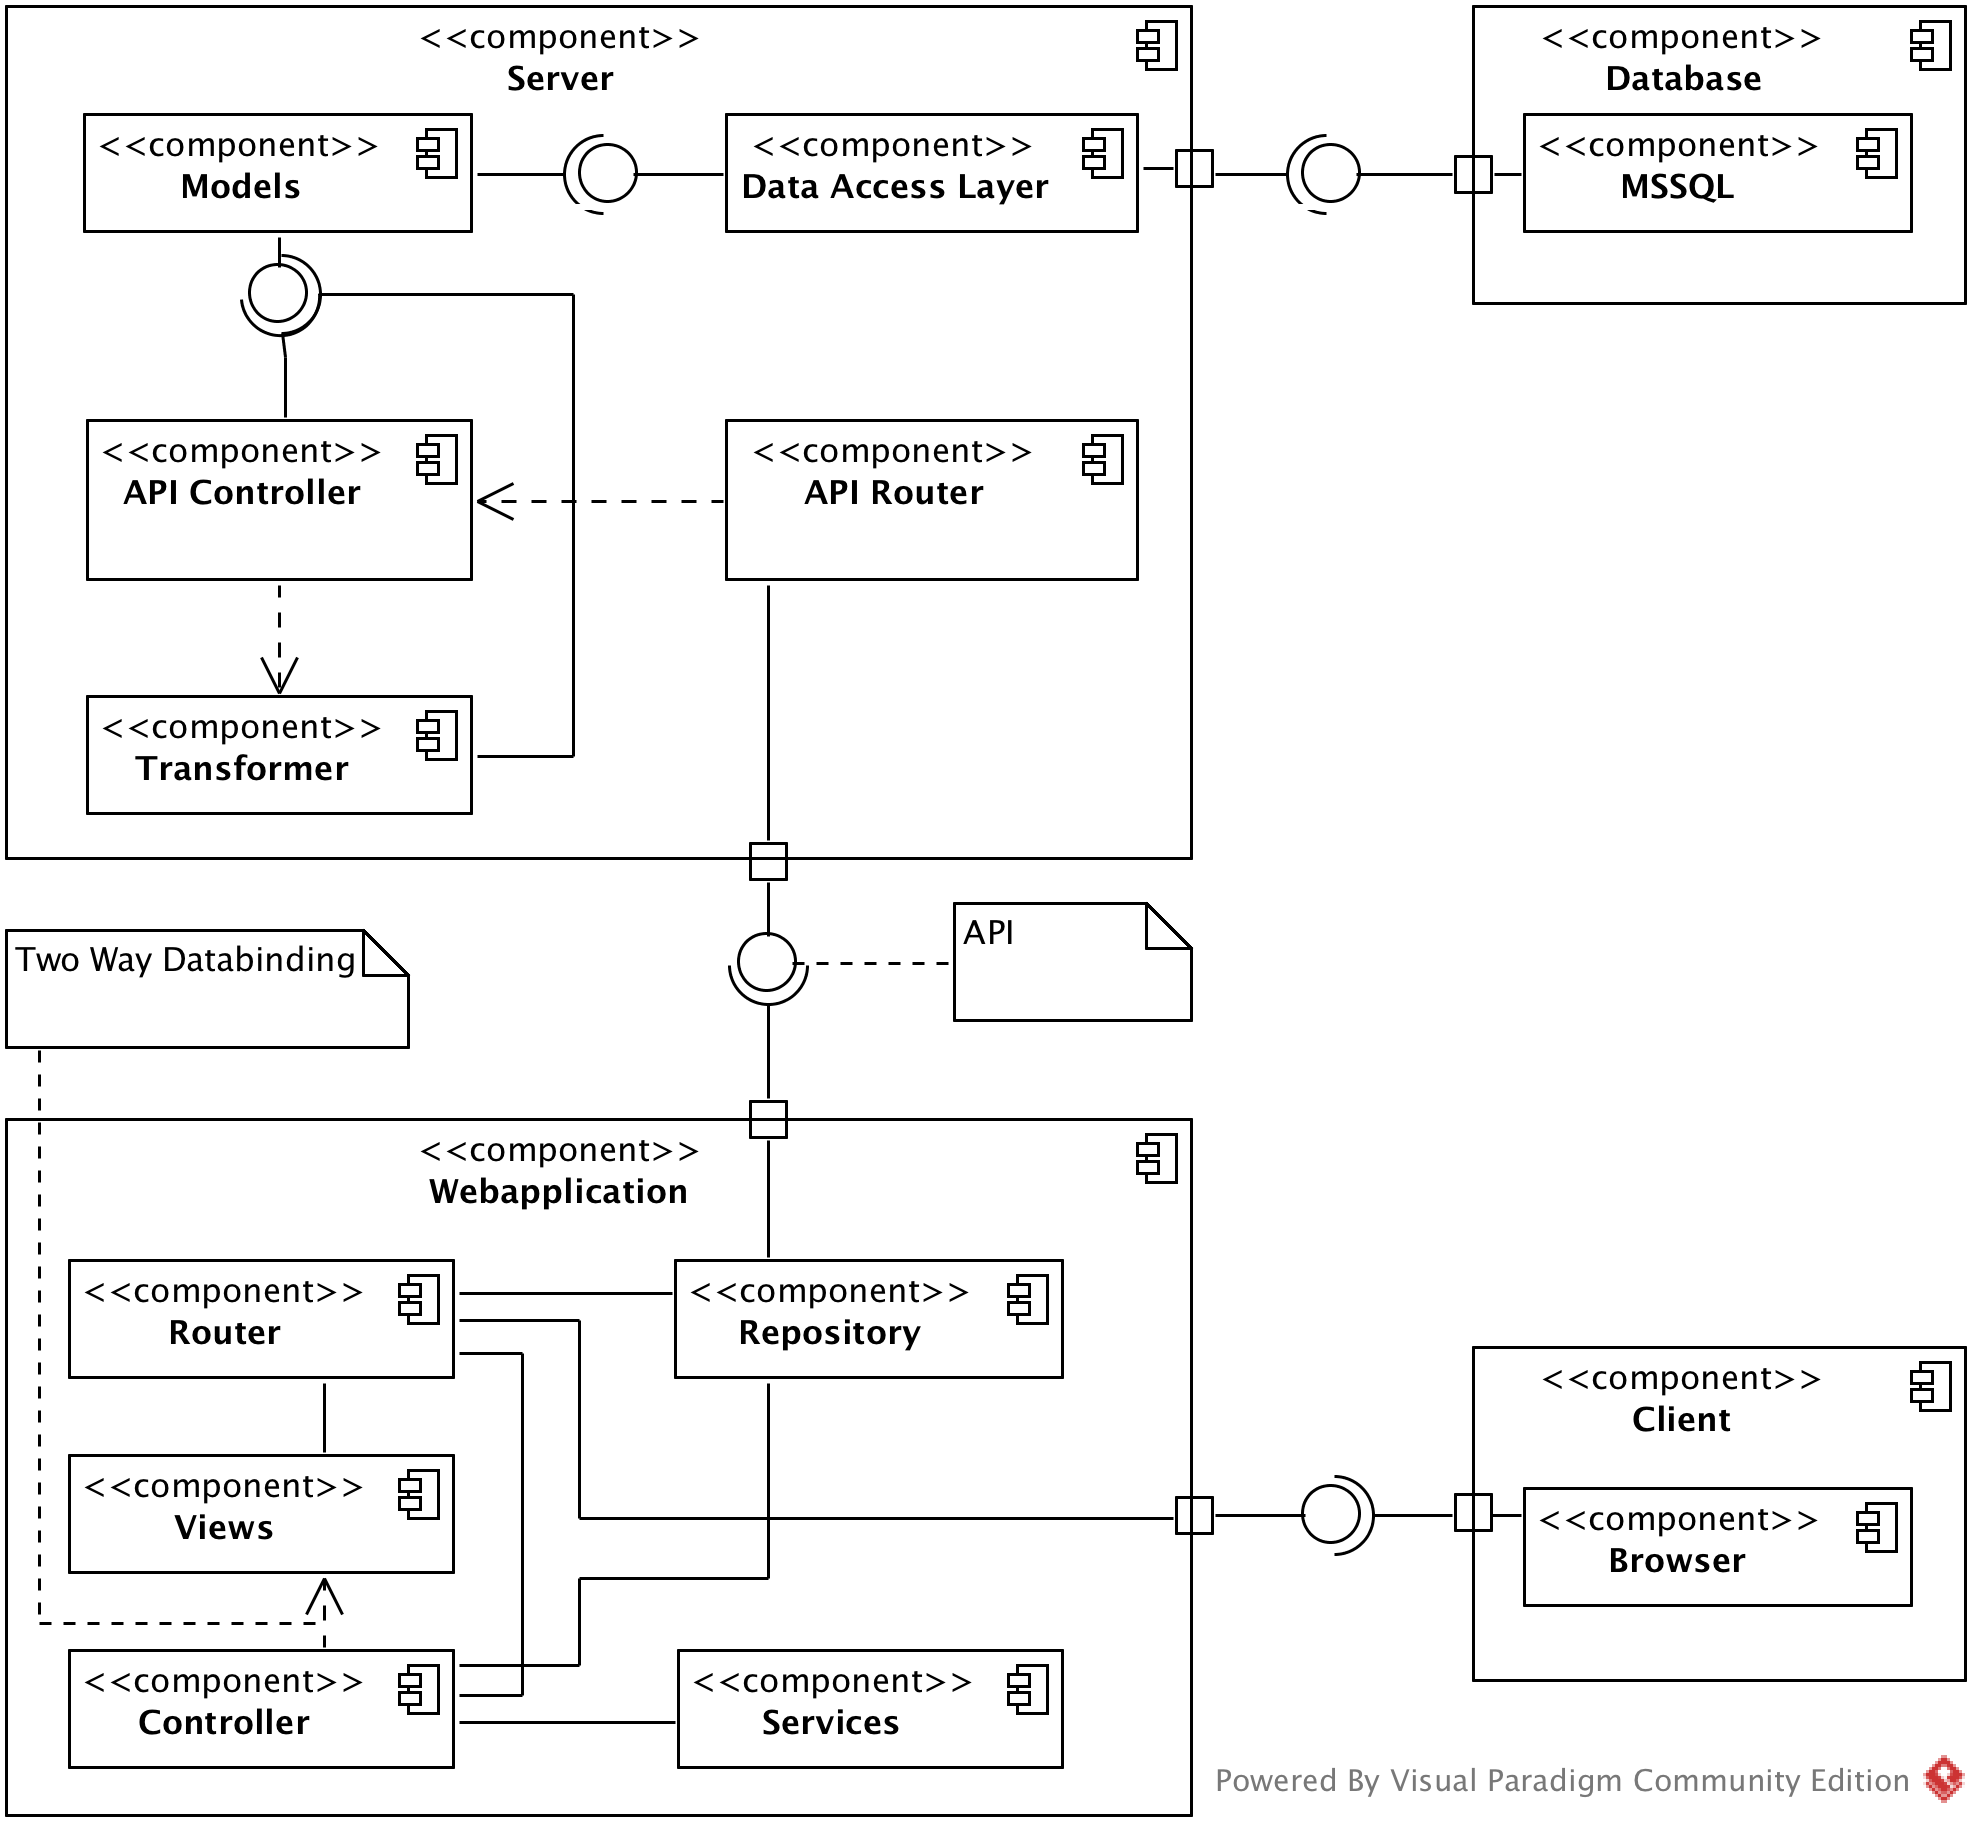
\includegraphics[width=1.0\textwidth]{architecture} %{CS0031}
\caption{Komponentendiagramm der Webanwendung}
\label{fig:architecture}
\end{figure}

\subsection{Server}
\label{sec:Entwurf:Server}

Hauptaufgabe des Server ist die Bereitstellung einer REST konformen Schnittstelle und die Realisierung einer Datenbankverbindung. Die Schnittstelle wird durch einen \emph{Router} implementiert, der alle aufrufbaren Endpunkte\footnote{Ein \acf{URI}, der einen eindeutigen Zugriff auf eine Ressource zulässt, wird auch als Endpunkt bezeichnet.} kapselt. Wird ein solcher Endpunkt aufgerufen, leitet der Router die Anfrage an einen zuständigen Controller weiter. Ein Controller implementiert Methoden, die die in Abschnitt \ref{sec:ROA:Einheitliche Schnittstelle} dargestellten HTTP-Methoden in ihrer Funktionsweise im Kontext einer REST konformen Schnittstelle widerspiegeln. Das bedeutet, dass die Controller im wesentlichen für die Realisierung typischer Funktionen (Lesen, Schreiben, Löschen, Aktualisieren), die auf einer Ressource ausgeführt werden können, zuständig sind. Die dabei benötigte Kommunikation mit der zur Verfügung gestellten Datenbank erfolgt über eine \emph{Datenzugriffsschicht}, die mittels eines ORM-Frameworks realisiert wird. Das ORM-Framework erlaubt es \emph{Models} zu definieren, die jeweils eine Datenbanktabelle als Objekt beschreiben. Modelklassen beinhalten neben dem Schema der Tabelle auch Beziehungen, die über vom ORM-Framework bereitgestellte Methoden modelliert werden. Die Controller implementieren diese Modelklassen, mit Hilfe derer ein Zugriff auf die Datenbank erfolgen kann. Bevor die abgefragten Daten aber als Antwort über die Schnittstelle zurückgeschickt werden, findet eine Standardisierung und Homogenisierung statt. Dieser Vorgang ist notwendig, weil ansonsten ungefilterte Daten aus der Datenbank übertragen werden würden, die vom aufrufenden Client für die Realisierung seiner Aufgaben unter Umständen nicht alle benötigt werden oder im falschen Format vorliegen. Aus diesem Grund implementieren die Controller zusätzlich noch so genannte \emph{Transformer}. Diese werden mit dem Ergebnis aus dem Aufruf der Modelklassen, also mit Rohdaten aus der Datenbank, aufgerufen. Die Transformer definieren, welche Daten in welcher Form im Bezug auf die Rohdaten über die Schnittstelle übertragen werden sollen. Bei diesem Prozess wird unter anderem auch das Datenformat der Übertragung festgelegt. Zusätzlich verfügen die Transformer auch noch über die Möglichkeit, aus denen in den Modelklassen definierten Beziehungen, Daten aus verknüpften Tabellen in die Antwort einzubetten. Ist dieser Prozess abgeschlossen, werden die Daten als Antwort über den Router zurück an den Client geschickt.

\subsection{Client}
\label{sec:Entwurf:Client}

Der Client wird als \ac{SPA} auf Basis des AngularJS Frameworks realisiert. Eine \ac{SPA} zeichnet sich durch ein einziges HTML-Dokument aus, in dem Inhalte dynamisch nachgeladen werden können. Diese Art der Webarchitektur steht im Gegensatz zu klassischen Webanwendungen, welche aus mehreren, untereinander verlinkten HTML-Dokumenten bestehen, die meist vom Server bereitgestellt werden. Als zentrale Komponente dient der Webanwendung, wie auch schon dem Server, ein \emph{Router}. Dieser Router kapselt alle aufrufbaren Routen der Webanwendung und wird durch den Aufruf einer \ac{URL} aus einem Browser heraus angesteuert. Der Router setzt sich aus sogenannten \emph{States} zusammen. Ein State definiert neben der \ac{URL} einen zugehörigen \emph{Controller} und \emph{View}. Nach dem Aufruf eines States wird der angegebene Controller aufgerufen und der zugehörigen View in Form eines HTML-Dokuments in das \ac{DOM} geladen. Die States haben außerdem die Möglichkeit, sogenannte \emph{Resolves} zu implementieren. Das sind Abhängigkeiten, die vor dem Aufruf des Controllers und der Anzeige der View aufgelöst werden. Resolves können zum Beispiel Schnittstellenaufrufe zum Laden benötigter Daten implementieren. Der Vorteil liegt dabei darin begründet, dass der View tatsächlich erst angezeigt wird, wenn alle benötigten Daten geladen wurden und damit keine unvollständigen Seiten angezeigt werden. Der Aufruf der Schnittstelle wird durch ein \emph{Repository} gekapselt, in dem alle verfügbaren Endpunkte definiert sind. Das Repository ist faktisch das Gegenstück des API-Routers auf der Serverseite. Der Aufruf der Schnittstelle erfolgt mittels \ac{AJAX}. Das asynchrone Laden der Daten, hat den wesentlichen Vorteil, dass die Webanwendung während des Ladevorgangs benutzbar bleibt. Daten die als Resolve bereitgestellt werden, werden vom Router automatisch in den entsprechenden Controller injiziert. Ein Controller im Kontext von AngularJS ist nichts weiter als eine normale Javascript-Funktion. Eine Besonderheit ist nur die übergebene Variable \$scope. Mit dieser Variable können Daten mit dem View über eine bidirektionale Datenbindung ausgetauscht werden. Eine wesentliche Aufgabe von Controllern ist demnach die Bindung von Daten (die zum Beispiel über die Schnittstelle kommen können) an die \$scope Variable, um sie im View nutzbar zu machen. Daten, die an den Scope gebunden werden, bezeichnet man auch als \emph{Models}. Damit realisiert die Webanwendung ein klassische \ac{MVC} Architektur als Teil einer \acf{ROA} - wenn man das große ganze betrachtet. Eine weitere Komponente der Webanwendung bilden \emph{Services}. Services sind Klassen oder Funktionen die Business-Logik auf der Clientseite implementieren. Services können generell von allen Komponenten der Webanwendung genutzt werden.

\section{Datenbankmodell}
\label{sec:Entwurf:Datenbankmodell}

Die zur Verfügung gestellt Datenbank umfasst die vollständige Datenbasis der FlowConfigurator Software. Für die Realisierung der Webanwendung werden aber nicht alle Datenbanktabellen benötigt. Das in Abbildung \ref{fig:erdiagram} erarbeitete Datenbankschema beinhaltet die für die Realisierung der Webanwendung benötigten Tabellen.

\begin{figure}[H]
\centering

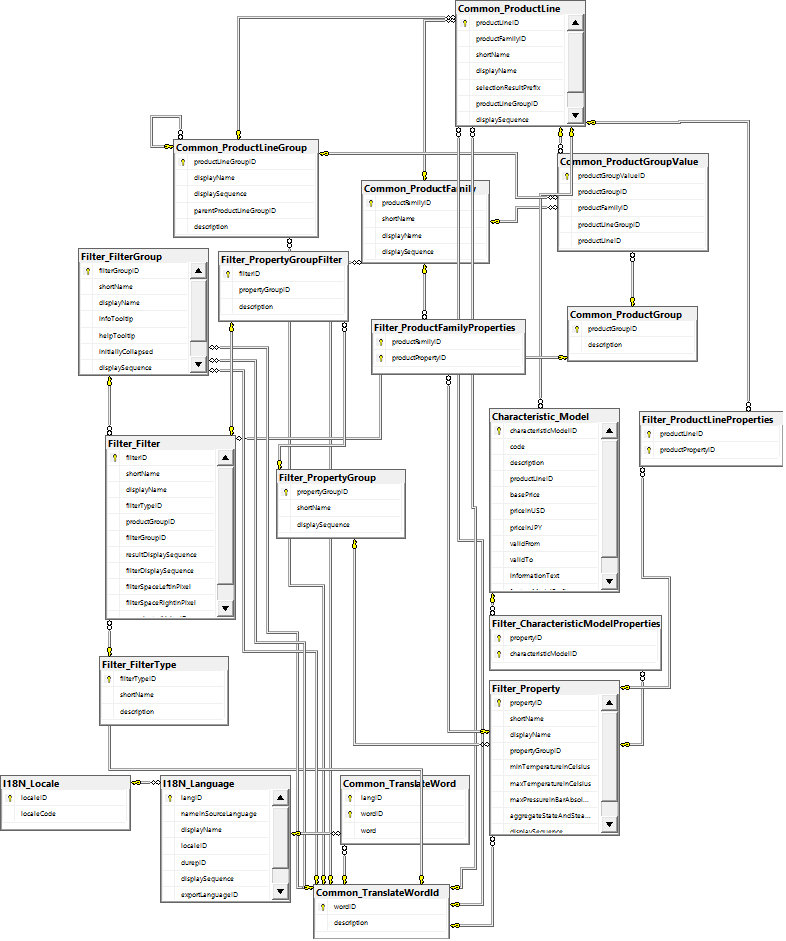
\includegraphics[width=1.0\textwidth]{er-diagram} %{CS0031}
\caption{Datenbankschema der Webanwendung}
\label{fig:erdiagram}
\end{figure}

Für das weitere Verständnis der Arbeit werden die ermittelten Tabellen nachfolgend aufgelistet und deren Inhalt und Beziehung beschrieben. Aufgrund der Komplexität der vorliegenden Datenstruktur kann dies nicht vollumfänglich und im Detail geschehen, sodass zusätzlich detailliertere Beschreibungen wichtiger Tabellen auch in aufbauenden Kapiteln erfolgen.

\subsubsection{Filter}

Die Filtertabelle ist die Ausgangstabelle der Filterabstraktion und beinhaltet layoutspezifische Daten zur Darstellung und Anordnung der Filtersteuerelemente. Ebenso werden Beziehungen zu FilterGroups, FilterTyps und PropertyGroupFilter hergestellt.

\subsubsection{FilterGroup}

Filtergruppen sind Bestandteil der layoutspezfischen Merkmale eines Filtersteuerelements. Es wird zwischen Basis- und erweiterten Filtern unterschieden. Diese Unterscheidung kommt bei der Anordnung der Filtersteuerelemente zum tragen.

\subsubsection{FilterTyp}

Ein Filtertyp bezeichnet die Ausprägung des Filtersteuerelements. Es wird zwischen Schaltern (Checkboxen) und Dropdown-Listen unterschieden.

\subsubsection{PropertyGroupFilter}

Die PropertyGroupFilter-Tabelle beschreibt eine Art der Filterung nach Properties. Sie ist eine Verknüpfungstabelle und stellt die Beziehung zur Filter-Tabelle und PropertyGroup-Tabelle her.

\subsubsection{PropertyGroup}

Die PropertyGroup-Tabelle beinhaltet übergreifende Sensormerkmale, nach denen gefiltert werden soll. Sie realisiert außerdem die Beziehung zur Property-Tabelle.

\subsubsection{Property}

Die Property-Tabelle beinhaltet konkrete Gerätevorgaben, d.h. Geräteeigenschaften, nach denen bei der Anwendung eines Filters entsprechend der Vorgabe passende Sensoren ermittelt werden.

\subsubsection{ProductLineProperty}

Bestimmte Geräteeigenschaften sind auf eine gesamte Produktlinie anwendbar. Die ProductLineProperty-Tabelle ist eine Verknüpfungstabelle und stellt die Beziehung zwischen einer Property und einer Produktlinie her.

\subsubsection{ProductFamilyProperty}

Wenige zu filternde Geräteeigenschaften treffen sogar auf alle Produkte innerhalb einer Produktfamilie zu. Die ProductFamilyProperty-Tabelle ist ebenfalls eine Verknüpfungstabelle, die die Beziehung zwischen einer Property und einer Produktfamilie realisiert.

\subsubsection{CharacteristicModel}

Die CharacteristicModel-Tabelle enthält die zu bestimmenden Models. Models beschreiben dabei Sensoren, die einer Produktlinie zugeordnet werden können. Als Besonderheit referenziert die CharacteristicModel-Tabelle auf sich selbst, so das Verschachtelungen der Models möglich sind.

\subsubsection{CharacteristicModelProperties}

Die CharacteristicModelProperties-Tabelle ist eine Verknüpfungstabelle, welche die Beziehung zwischen einer Property und einem CharacteristicModel realisiert. Sie beinhaltet also die Information, welche spezifizierten Geräteeigenschaften tatsächlich auf ein oder mehrere CharacteristicModels anwendbar sind.

\subsubsection{ProductFamily}

Produkte werden kategorisiert und gehören unter anderem einer Produktfamilie an. Die ProductFamily-Tabelle realisiert die Beziehung zu Produktgruppen und Produktlinien, als eine speziellere Art der Kategorisierung von Produkten. Produktfamilien werden im Kontext dieser Arbeit auch als Technologien bezeichnet.

\subsubsection{ProductLineGroup}

Als eine feingranulare Art der Kategorisierung beschreibt die ProduktLineGroup-Tabelle die Zusammenfassung von Produktlinien in bestimmte Gruppen. Es gibt Produktlinien, die keiner Produktliniengruppe angehören und direkt mit einer Produktfamilie verknüpft sind.

\subsubsection{ProductLine}

Eine Produktlinie ist in der hierarchischen Strukturierung von Produkten die feinste Art der Kategorisierung. Die ProductLine-Tabelle realisiert die Beziehung zu CharacteristicModels.

\subsubsection{ProductGroup}

Eine Produktgruppe beschreibt eine weitere Art der Kategorisierung, die sich aber nicht als Teil der hierarchischen Strukturierungen versteht. Zudem ist die Produktgruppe der logische Zusammenschluss aus einer Produktfamilie, Produktliniengruppe und Produktlinie oder auch nur Teilen davon. Auch ist eine Produktgruppe ein wichtiger Bestandteil der Datenstruktur, da die ProductGroup-Tabelle die Beziehung zur Filter-Tabelle herstellt.

\subsubsection{ProductGroupValues}

Die ProductGroupValues-Tabelle ist eine Verknüpfungstabelle, welche die zuvor beschriebene Beziehung zwischen einer Produktfamilie, Produktliniengruppe und Produktlinie zu einer Produktgruppe herstellt.

\subsubsection{TranslateWordId}

Um die Mehrsprachigkeit der FlowConfigurator Software zu realisieren, werden alle Wörter und Bezeichnungen in der Datenbank gespeichert. Es liegen jeweils Übersetzungen in mehreren Sprachen vor.

\subsubsection{TranslateWord}

Die TranslateWord-Tabelle ist eine Verknüpfungstabelle, welche die Beziehung zwischen einer Übersetzung und der zugeordneten Sprache herstellt.

\subsubsection{Language}

Die Language-Tabelle enthält alle verfügbaren Sprachen für die es möglich ist Übersetzungen anzulegen.

\section{Schnittstelle}
\label{sec:Entwurf:Schnittstelle}

Die zu entwickelnde Schnittstelle bildet die Basis der Kommunikation zwischen Server und Client. Ziel ist der Entwurf einer REST-konformen Schnittstelle, die die benötigten Daten zur Realisierung der in Abschnitt \ref{sec:Funktionale Anforderungen} aufgestellten funktionalen Anforderungen bereitgestellt. Dabei werden die in Abschnitt \label{sec:ROA:Prinzipien einer Ressource-Oriented Architecture} betrachteten Prinzipien einer \acf{ROA} berücksichtigt. Insbesondere die Zusammenfassung der in Abschnitt \ref{sec:Entwurf:Datenbankmodell} dargestellten Datenbasis als abstrakte Ressourcen eines REST-konformen Webservice und die damit verbundene Modellierung von nachvollziehbaren Ressourcenbezeichnern (\ac{URI}) ist Schwerpunkt des Entwurfs. In Tabelle \ref{tab:api} wird die ermittelte Schnittstellenspezifikation dargestellt und anhand der jeweils anwendbaren HTTP-Methoden beschrieben.

\begin{table}[H]
\centering
\def\rr{\rightskip=0pt plus1em \spaceskip=.3333em \xspaceskip=.5em\relax}
\setlength{\tabcolsep}{1ex}
\def\arraystretch{1.20}
\setlength{\tabcolsep}{1ex}
\small
\begin{tabular}{|p{0.29\textwidth}|p{0.12\textwidth}|p{0.65\textwidth}|}
\hline
   \multicolumn{1}{|c}{\emph{URI}} &
   \multicolumn{1}{|c}{\emph{Methode}} &
   \multicolumn{1}{|c|}{\emph{Beschreibung}} \\
\hline\hline
   {\rr /technologies} &
   GET &
Liefert alle Produktfamilien (Technologien).
   \\
\hline
   {\rr /technologies/\{id\}} &
   GET &
Liefert eine Produktfamilie (Technologie).
   \\
\hline
   {\rr /technologies/\{id\}/\break{}
   productlines} &
   GET &
Liefert alle Produktlinien und zugehörige Produktliniengruppen, die einer bestimmten Produktfamilie angehören.
   \\
\hline
   {\rr /technologies/\{id\}/\break{}
   productlines/\{id\}} &
   GET &
Liefert eine Produktlinie und zugehörige Produktliniengruppe, die einer bestimmten Produktfamilie angehört.
   \\
\hline
   {\rr /technologies/\{id\}/\break{}
   productlines/\{id\}/\break{}
   filters} &
   GET &
Liefert alle Filter und zugehörige Filtertypen, Filtergruppen, Produktgruppen, Filterarten die einer bestimmten Produktfamilie und Produktlinie angehören.
   \\
\hline
   {\rr /productgroups} &
   GET &
Liefert alle Produktgruppen.
   \\
\hline
   {\rr /filters} &
   GET &
Liefert alle Filter und zugehörige Filtertypen, Filtergruppen, Produktgruppen, Filterarten.
   \\
\hline
   {\rr /filters} &
   POST &
Legt einen neuen Filter an. Die Schnittstelle erwartet ein Filterobjekt inklusive zugehörigem Filtertyp, Filtergruppe, Produktgruppe und Filterart.
   \\
\hline
   {\rr /filters} &
   PUT &
Aktualisiert mehrere Filter. Die Schnittstelle erwartet mehrere Filterobjekte inklusive zugehöriger Filtertypen, Filtergruppen, Produktgruppen und Filterarten.
   \\
\hline
   {\rr /filters/\{id\}} &
   GET &
Liefert einen Filter und zugehörigen Filtertyp, Filtergruppe, Produktgruppe, Filterart anhand der übergebenen ID.
   \\
\hline
   {\rr /filters/\{id\}} &
   PUT &
Aktualisiert einen Filter mit einer bestimmten ID. Die Schnittstelle erwartet ein Filterobjekt inklusive zugehörigem Filtertyp, Filtergruppe, Produktgruppe und Filterart.
   \\
\hline
   {\rr /filters/\{id\}} &
   DELETE &
Löscht einen Filter anhand der übergebenen ID.
   \\
\hline
   {\rr /filters/\{id\}/\break{}
   properties/\{id\}/models} &
   GET &
Liefert alle Models und zugehörige Kind-Models, die einer bestimmten Property und Filter zugeordnet sind.
   \\
\hline
   {\rr /filters/types} &
   GET &
Liefert alle Filtertypen.
   \\
\hline
   {\rr /filters/types/\{id\}} &
   GET &
Liefert einen Filtertyp anhand der übergebenen ID.
   \\
\hline
   {\rr /filters/groups} &
   GET &
Liefert alle Filtergruppen.
   \\
\hline
   {\rr /filters/groups/\{id\}} &
   GET &
Liefert eine Filtergruppe anhand der übergebenen ID.
   \\
\hline
   {\rr /filters/properties/} &
   GET &
Liefert alle Properties.
   \\
\hline
   {\rr /filters/properties/\{id\}} &
   GET &
Liefert eine Property anhand der übergebenen ID.
   \\
\hline
   {\rr /filters/properties/\{id\}} &
   PUT &
Aktualisiert ein Property mit einer bestimmten ID. Die Schnittstelle erwartet ein Propertyobjekt.
   \\
\hline
   {\rr /filters/properties/\{id\}} &
   PUT &
Aktualisiert ein Property mit einer bestimmten ID. Die Schnittstelle erwartet ein Property-Objekt.
   \\
\hline
   {\rr /models} &
   GET &
Liefert alle Models inklusive Kind-Models
   \\
\hline
   {\rr /models/\{id\}} &
   GET &
Liefert ein Model inklusive Kindmodel anhand der übergebenen ID.
   \\
\hline
\end{tabular}
\caption{Schnittstellenspezifikation des konzipierten RESTful Webservice}
\label{tab:api}
\end{table}



\section{Benutzeroberfläche}
\subsection{Identifizierung benötigter Layout-Komponenten}
\label{sec:Analyse:Identifizierung von Layout-Komponenten}

In Abschnitt \ref{sec:Analyse:Benutzbarkeit und Layout} wurden als nichtfunktionale Anforderung bereits Aussagen über die Gestaltung der Benutzeroberfläche getroffen. Dabei wurde festgestellt, dass die zu gestaltende Benutzeroberfläche der Webanwendung, die für die im Kontext der Filterbearbeitung wichtigen Layout-Komponenten, der FlowConfigurator Software, übernehmen soll. Dabei geht es keinesfalls darum eine exakte Kopie des Layout zu entwickeln, sondern den \grqq{}Look and Feel\grqq{} der FlowConfigurator Software aufzugreifen und an die Bedürfnisse der Webanwendung anzupassen. Zu diesem Zweck werden in Abbildung \ref{fig:layout} unter Zuhilfenahme eines Screenshots der FlowConfigurator Software wichtige Layout-Komponenten identifiziert und nachfolgend der Transfer auf das Layout der Webanwendung diskutiert.

\begin{figure}[H]
\centering
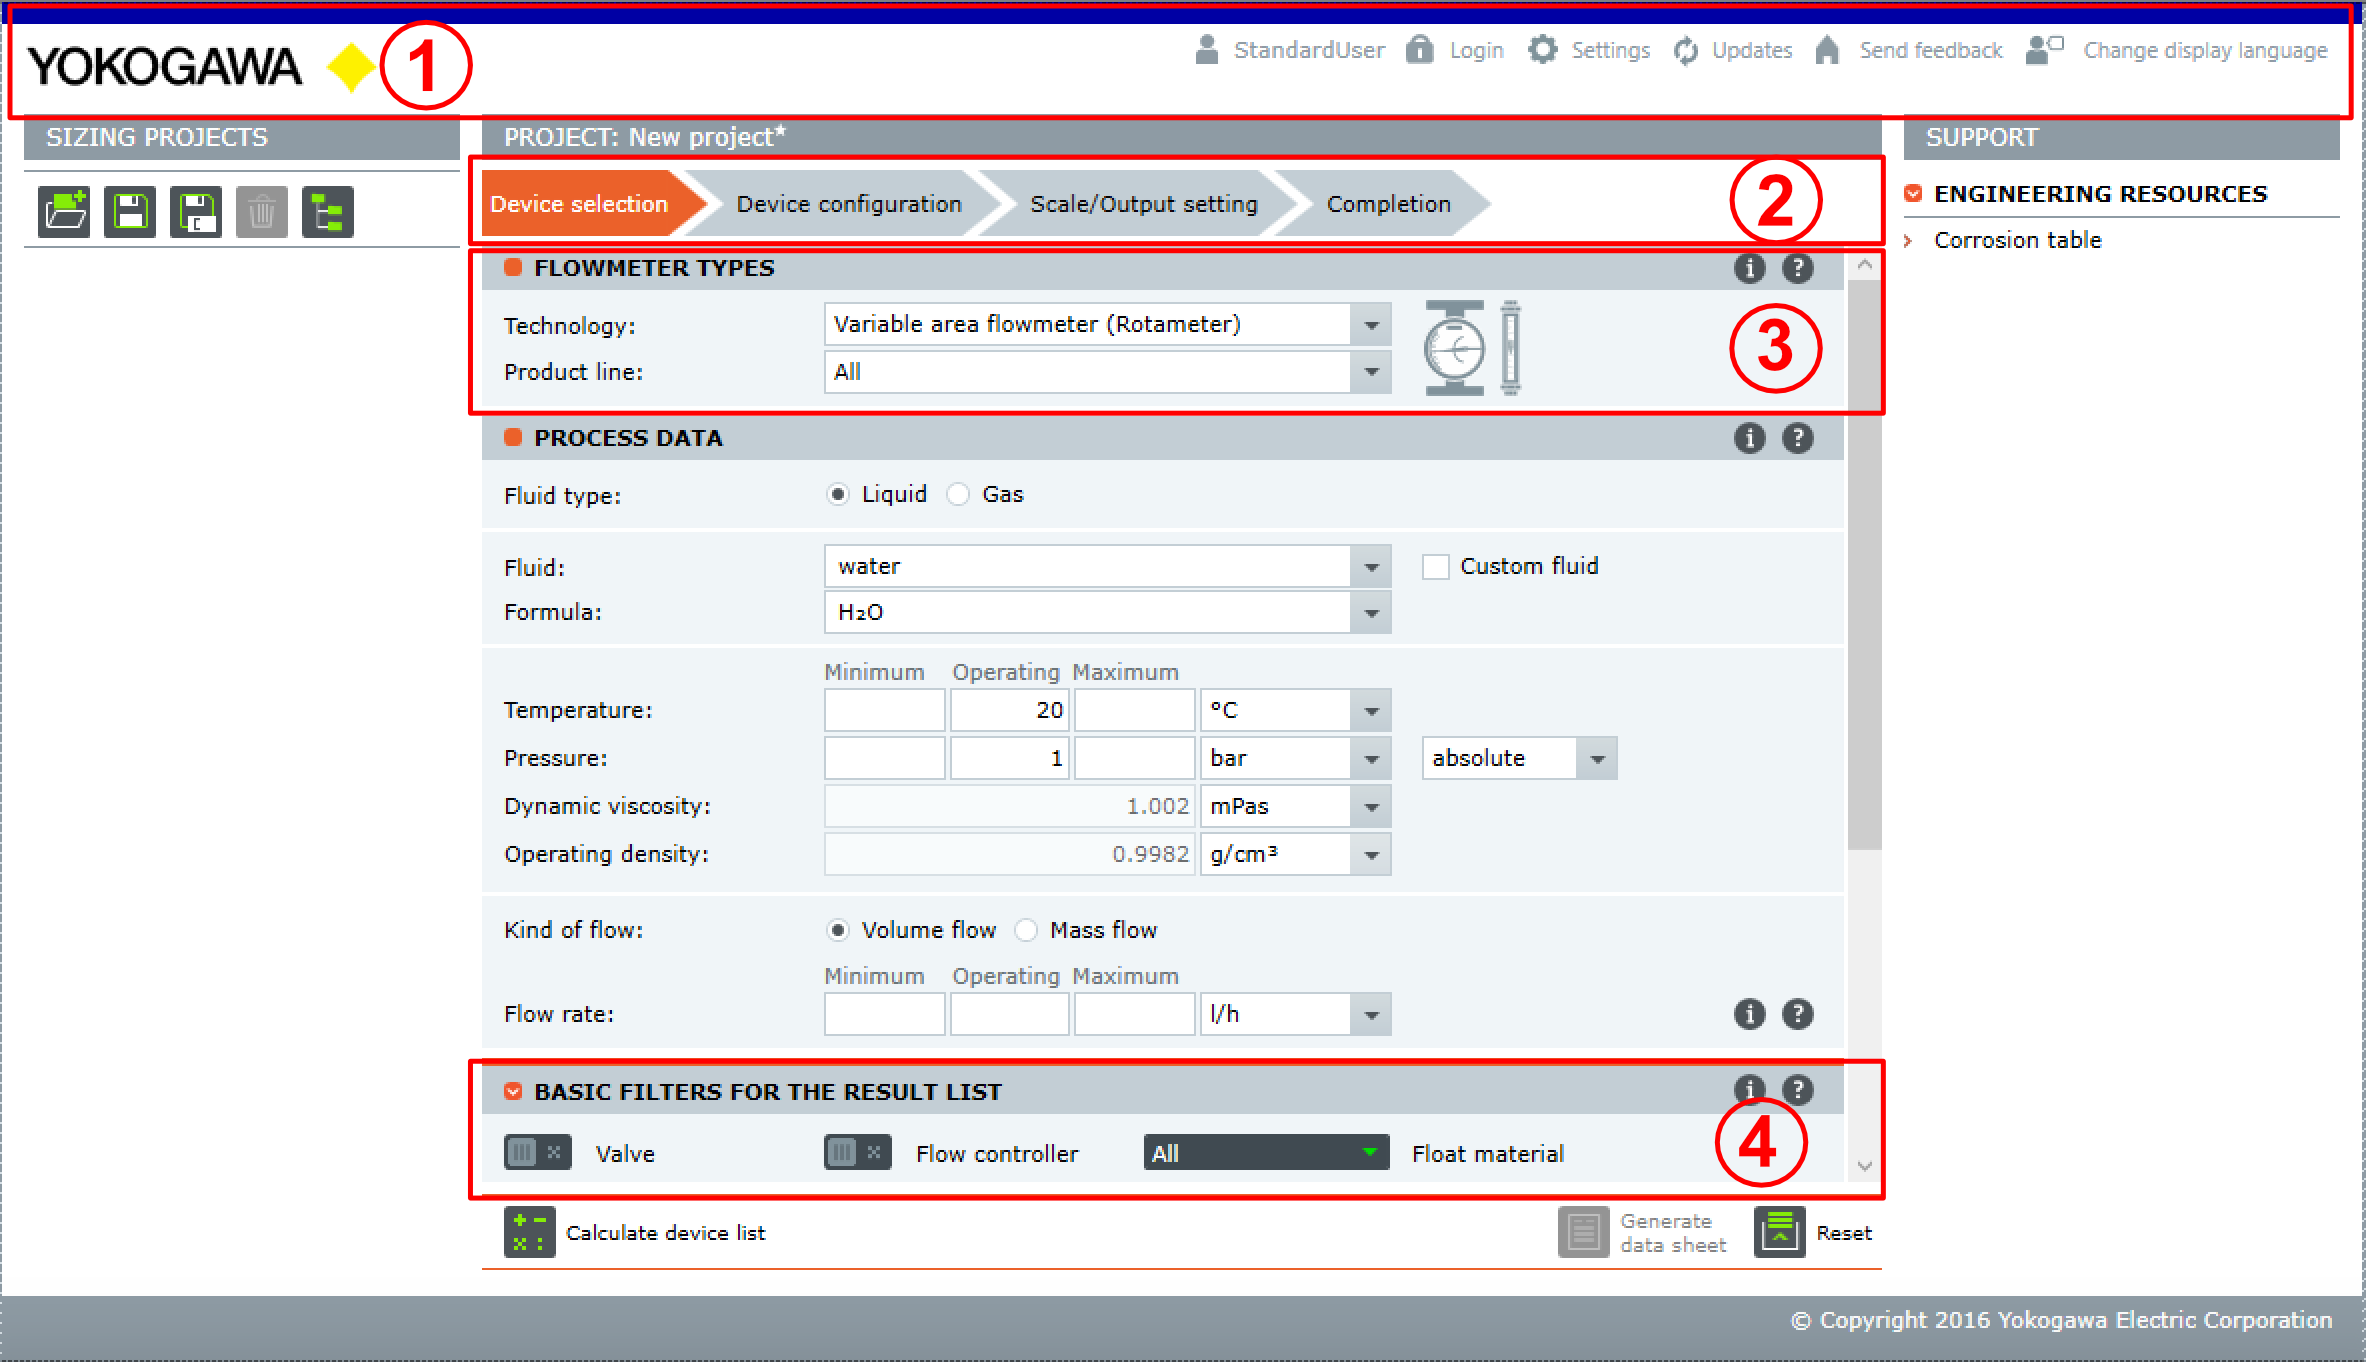
\includegraphics[width=.95\textwidth]{layout}
\caption{Identifizierung benötigter Layout-Komponenten zur Realisierung der Webanwendung}
\label{fig:layout}
\end{figure}

\subsubsection{{\larger\textcircled{\smaller[2]1}} Kopfzeile}

Die Kopfzeile zeigt dem Nutzer unter anderem an, ob er an der Applikation angemeldet ist und wenn ja unter welchem Benutzernamen. Diese Information ist ebenso für die Webanwendung relevant, da sich ein Benutzer auch an dieser anmelden muss.

\subsubsection{{\larger\textcircled{\smaller[2]2}} Navigationsassistent}

Anhand der Navigationsassistenten kann der Benutzer bestimmen, in welchem Schritt er sich bei der Gerätekonfiguration befindet und zusätzlichen bei Bedarf auch zwischen einzelnen Schritten navigieren. Die Webanwendung verfolgt mit der Bearbeitung der Filterdaten ein ähnliches Konzept, da auch diese aufgrund der Datenstruktur nur in mehreren Teilabschnitten zu bearbeiten sind. Aus diesem Grund, soll auch die Webanwendung eine ähnlich geartete Navigation realisieren.

\subsubsection{{\larger\textcircled{\smaller[2]3}} Technologie- und Produktlininenauswahl}

Anhand der bereitgestellten Dropdown-Listen schränkt der Benutzer den zu konfigurierenden Gerätetyp ein. Die getroffene Auswahl hat Auswirkungen auf die zur Verfügung stehenden Filter und muss damit auch als wichtiger Bestandteil der Webanwendung übernommen werden.

\subsubsection{{\larger\textcircled{\smaller[2]4}} Anzeige der Filtersteuerelemente}

Die Filtersteuerelemente werden auf Grundlage der in {\larger\textcircled{\smaller[2]3}} getroffenen Auswahl angezeigt. Auf dem Screenshot nicht zu sehen ist die zusätzliche Unterscheidung in Basis- und Spezialfiltern. Diese Layout-Komponente ist auch ein wesentlicher Kernbestandteil der Webanwendung, da hier die Filtersteuerelemente angezeigt werden, auf denen sich verschiedene Aktionen ausführen lassen sollen.

%
%\subsection{Benutzerführung}
%\begin{itemize}
%\item Wie funktioniert die Navigation auf der Seite mit Bezug auf das Layout
%\item Breadcrumb-Navigationshilfe erwähnen
%\item URL-Parameter steuern indirekt API (z.b. %ydm.de/filters/1 holt den Filter mit der ID 1 aus der %Datenbank und stellt Daten in einer Detailansicht dar)
%\item User Feedback Elemente und deren Einfluss auf die %Nutzerführung erläutern (Messages, Ladeanimationen etc.)
%\end{itemize}

\subsection{WYSIWYG als Gestaltungskonzept}
\label{sec:Entwurf:WYSIWYG als Gestaltungskonzept}

Dieser Abschnitt beschäftigt sich mit dem WYSIWYG-orientierten Gestaltungskonzept als ein Bestandteil der Benutzeroberflächengestaltung der Webanwendung. WYSIWYG beschreibt in seinem Kern einen Vorgang, bei dem Objekte durch den Benutzer mithilfe eines wie auch immer ausgeprägten Editors bereits so dargestellt bzw. bearbeitet werden können, wie sie dann später im \grqq{}Echteinsatz\grqq{} ebenfalls für den Benutzer der Anwendung erscheinen. Verfügbare Funktionen werden beispielsweise mit Hilfe von Steuerelementen an diesen Objekten angeboten; können dort vom Benutzer ausgewählt und auf einer Arbeitsfläche mithilfe direkter Manipulation, beispielsweise im Drag-and-Drop-Modus, verändert werden. Typische Anwendungsgebiete sind zum Beispiel WYSIWYG-Texteditoren, die es erlauben einen Text so zu formatieren, wie er später auch präsentiert wird (zum Beispiel im Druck, oder als ein Beitrag auf einer Webseite). Die angestrebte Funktionsweise der Webanwendung baut demnach auf ein sehr ähnliches Prinzip. An Stelle der eben als Beispiel genannten Texte treten komplexe Filterdaten auf, die als Filtersteuerelemente in der Benutzeroberfläche sichtbar sind. Anstatt Texte zu formatieren, soll die Ausprägung und Anordnung der Filtersteuerelemente auf einer Arbeitsfläche veränderbar sein. Dies kann aufgrund der komplexen Datenbasis natürlich nicht ausschließlich durch direkte Manipulation der Filtersteuerelemente geschehen. Es geht dabei vielmehr um den Teil der Filterdaten, welche das Aussehen und die Anordnung der Filtersteuerelemente bestimmen. Die Anordnung der Filtersteuerelemente lässt sich beispielsweise nur sinnvoll anpassen, wenn der Benutzer bei diesem Vorgang die Relation zu den umgebenden Filtersteuerelementen nicht verliert. Deshalb wird für die Webanwendung ein interaktiver Drag-and-Drop-Mechanismus konzipiert. Der Benutzer kann in der Webanwendung Filtersteuerelemente anklicken und diese frei in einem vorgegebenen Grid-System (Arbeitsfläche) verschieben. Das Ergebnis dieses Prozesses wird dann repräsentiert als Datenstruktur abgespeichert. Das bedeutet, dass die Funktionalität die für die Bearbeitung der Filtersteuerelemente realisiert wird, bereits einen - wenn auch nicht sehr ausgeprägten - WYSYWIG-Editor beschreibt.

WYSWYIG lässt sich aber außerdem noch, auf einen weiteren Aspekt des Systems übertragen. Auch wenn die Analogie etwas hinkt, lässt sich auch die Webanwendung als Ganzes als eine Art WYSIWYG-Editor betrachten. Die komplette Funktionalität der Webanwendung ist letztendlich darauf ausgerichtet Filterdaten zu bearbeiten, die zum Teil durch die angezeigten Filtersteuerelemente in der Benutzeroberfläche sichtbar gemacht werden. Durch den Export der Daten als Mittel zur Wiedernutzbarmachung in der FlowConfigurator Software ergibt sich damit ein ähnliches \ac{WYSIWYG}-Konstrukt, das bereits durch das vorangegangene Texteditor Beispiel aufgezeigt wurde. Der Vergleich ist nur deshalb nicht ganz sauber, weil aufgrund der Komplexität der zugrunde liegenden Daten nur wenige Teilbereiche der Bearbeitung tatsächlich auf direkte Manipulation von Objekten beruhen\footnote{Die direkte Manipulationen von Objekten ist ein oft genanntes Merkmal wenn von WYSIWYG-Systemen gesprochen wird, faktisch aber keine Grundvoraussetzung.}. Nichtsdestotrotz trägt auch dieser Aspekt zum Verständnis der Webanwendung als WYSIWYG-orientiertes System bei.




